\section{Implementation}
Development of OSM started with development in phases which focus on particular need of project.
Various phases and their detail are given below -:
\begin{itemize}
\item Phase I (Setup OSM Server) -: \\
        During Phase I, install all the dependecies(components) as mentioned above to make your own osm tile sever. After installing the softwares download the map in pbf(may be osm) format and render your own tile server. You can see your map on the browser after moving to the location which is being downloaded.

\begin{figure}[ht]
\centering 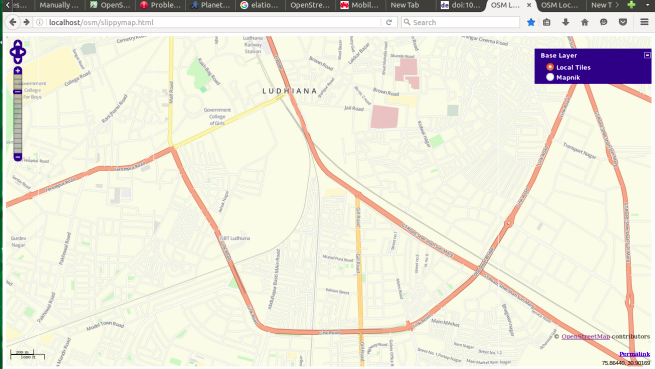
\includegraphics[width=0.7\textwidth]{input/images/osm7.png}
\caption{OSM Map on Web browser}
\end{figure}

\item Phase II (Styling of Map) -: \\
        During phase II, there is a lot of customization as listed below:-
\begin{itemize}
\item Colors of the buildings, roads, primary lines, secondary lines etc have been customized and then re-render the map to view the changes in the map.
\begin{figure}[ht]
\centering 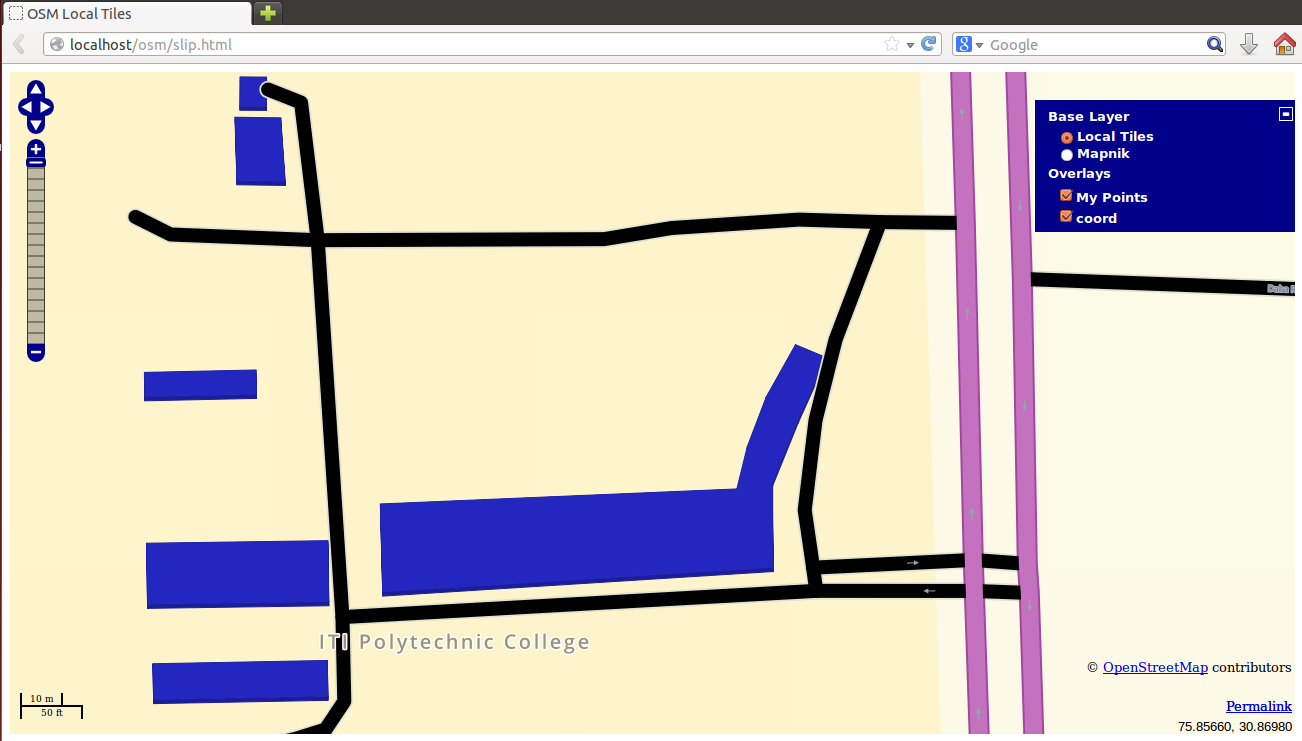
\includegraphics[width=0.7\textwidth]{input/images/osm5.png}
\caption{Map Styling}
\end{figure}

\item Added international boundary of India with customizable color and pixels.
\item Modified the icons of the nodes.
\item Customize the language of the map by applying Algorithm- if Punjabi name is provided then first priority goes to it followed by hindi and then English.
\item Admin levels at different zoom levels with different colors.	
\item Display name of the places over each places.

\item Phase III (Increased zoom levels to 28 for indoor mapping) -: \\
	        The purpose of phase III was to increase the zoom levels to more than 19 so to create the space for indoor mapping. It is done in mod\_tile module by applying another different algorithm. 
		\begin{figure}[ht]
			\centering 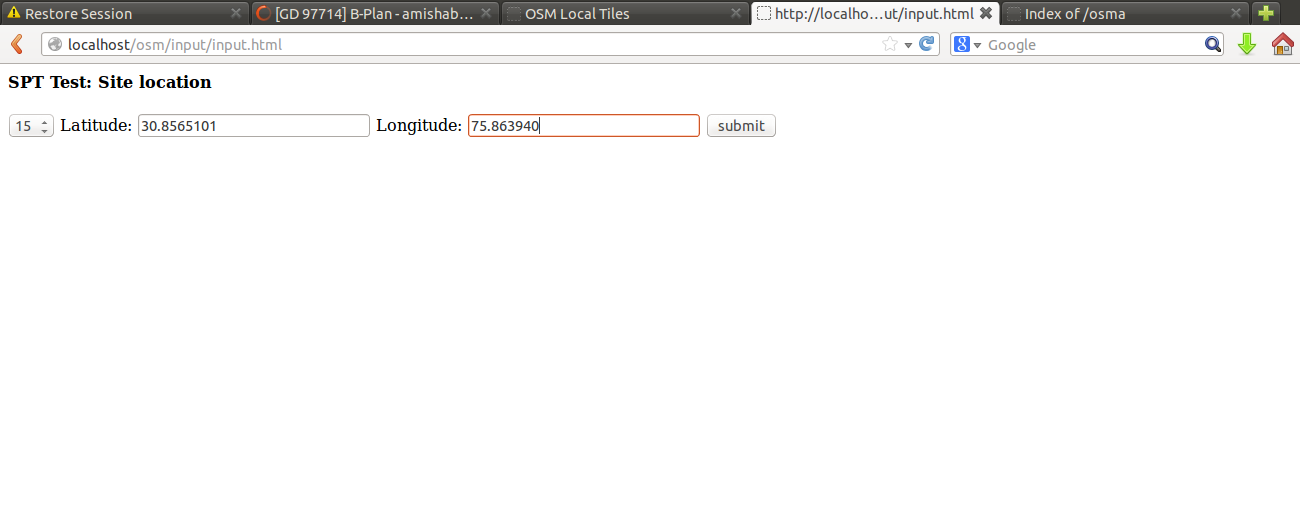
\includegraphics[width=0.7\textwidth]{input/images/osm2.png}
			\caption{User Input Page}
		\end{figure}

\item Phase III (User Input Map) -: \\
        During phase III, we made the html and php pages in which user can input latitude, longitude and zoom level of his own choice and if the tile image of that location is downloaded then on one click the map of that particular location will be visible. The functioning is done with the help of Javascript.
\begin{figure}[ht]
\centering 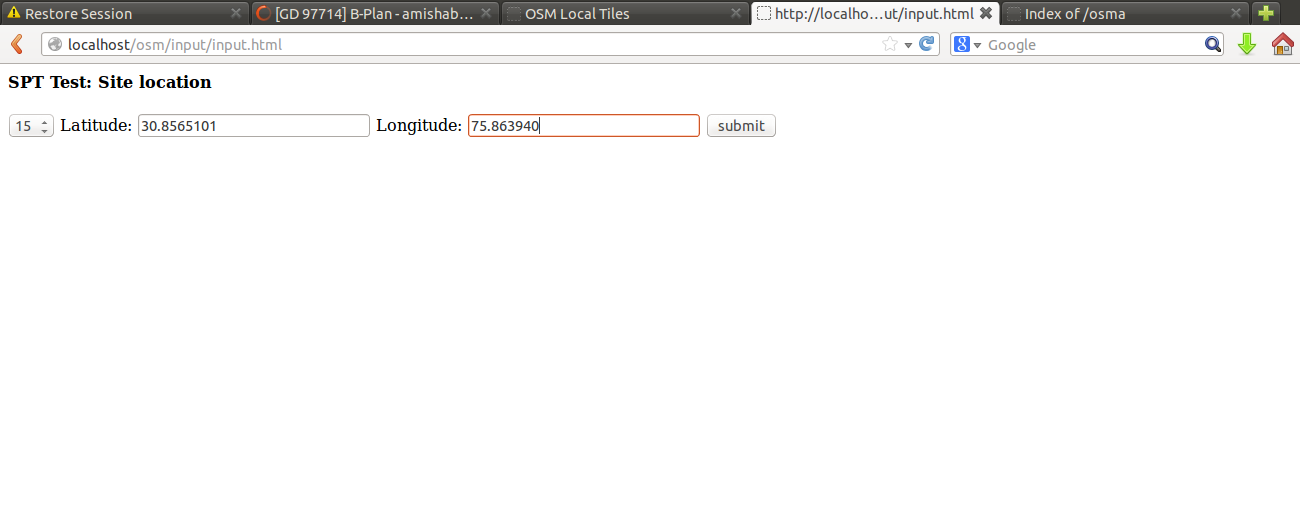
\includegraphics[width=0.7\textwidth]{input/images/osm2.png}
\caption{User Input Page}
\end{figure}

\begin{figure}[ht]
\centering 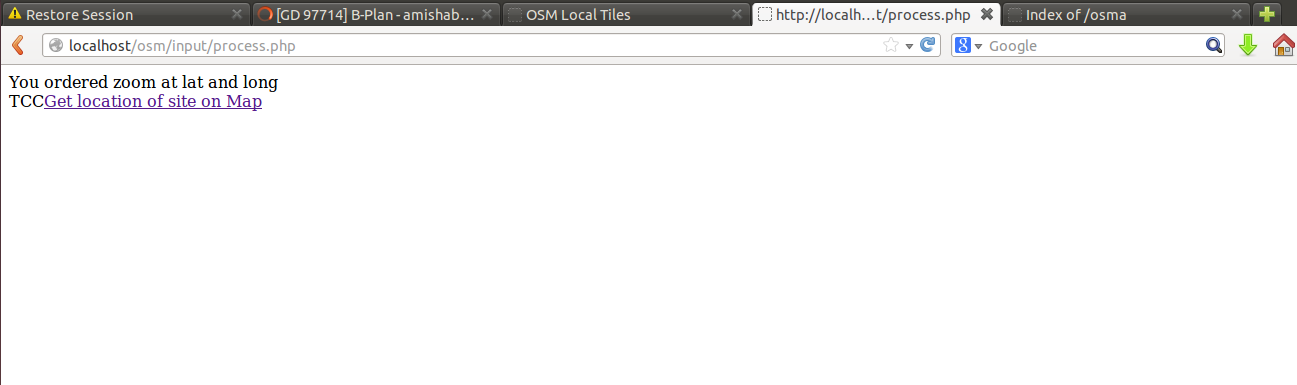
\includegraphics[width=0.7\textwidth]{input/images/osm3.png}
\caption{Php Page}
\end{figure}

\item Phase IV (Configurable OSM Installation Script) -: \\
	Building your system as an OSM server, is standalone task that can acquire atleast 15 days for beginner. So the purpose for phase IV is to make a script as easy Wordpress Installation. It is the shell non- interactive, one time configurable script (user have to change hardly two three parameters inside it) at the initial stage and then can run the script and can go for a cup of coffee.

\item Phase V (Event Handling) -: \\
During phase V, we tried to control the movement of the osm map through the arrow keys of keyboard and we achieved it. Again it is done with the help of Javascript with the concept of event handling. Various formulas are being applied and testing have been done while doing it. The code for the same is on the experimental server. Now, the map can be controlled through arrow keys also. Isn't it amazing. 

\item Phase VI (Insert Pop up Menu and Icons) -: \\
During phase VI, we added textfile containing different attributes like lat, lon, icon etc. At a particular location(through lat and lon) an icon in the form of image showing some message(Pop-up menu mostly with the name of shops at that location). The all points can be disable by disabling the layer "My Points". 
\begin{figure}[ht]
\centering 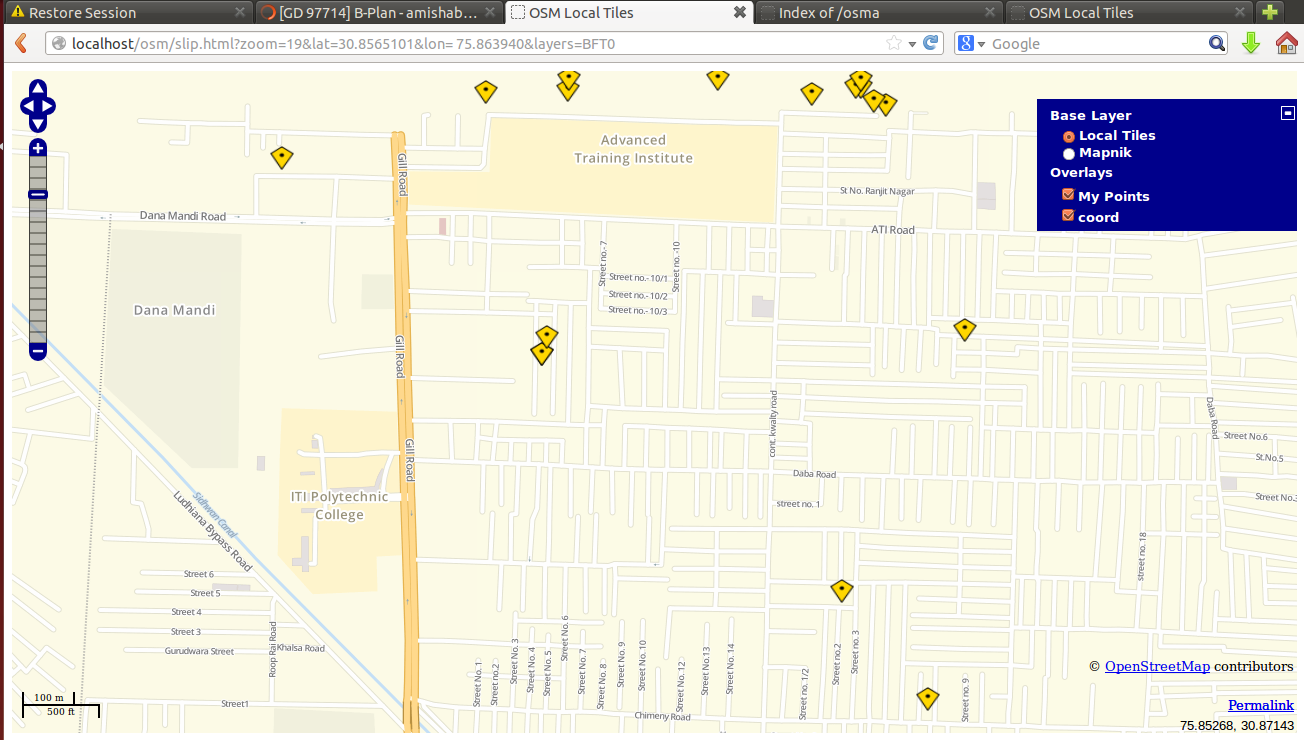
\includegraphics[width=0.7\textwidth]{input/images/osm1.png}
\caption{Map with pop-up menu and icons}
\end{figure}

\item Phase VII (Map On Remote Server) -: \\
During phase VII, we have added all the things above in the experimental account. It is done so that everyone can see it and for back up purpose also so that the code and project retains on other system also.
\begin{figure}[ht]
\centering 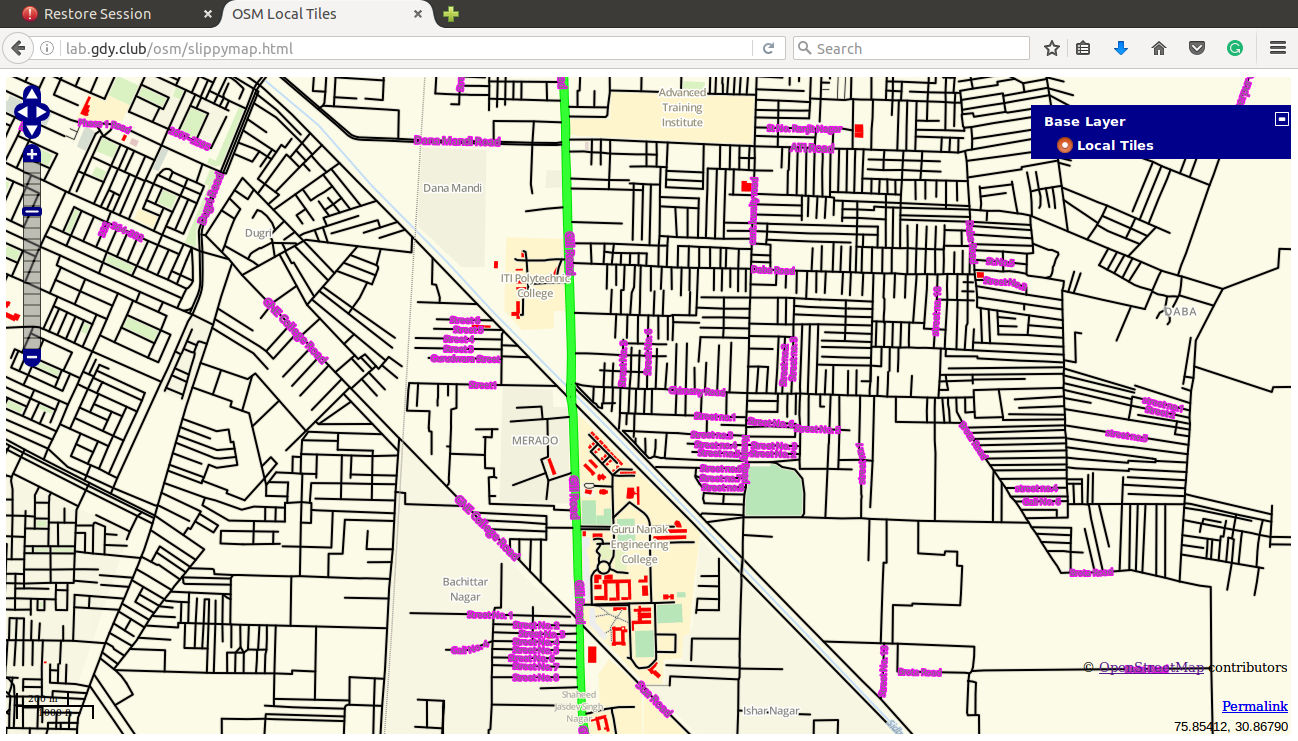
\includegraphics[width=0.7\textwidth]{input/images/osm8.png}
\caption{Map on remote server}
\end{figure}

\item Phase VI (Documentation) -: \\
During final phase, we documented the project( developers documentation and README.md)
using doxygen and wrote the report for this software.
\end{itemize}

\section{Animation}
On selecting animation a list of animations will appear, on selecting any of the place the page will move to the selected geolocation. view.animate() is used to add one or more animations.

\begin{figure}[ht]
\centering 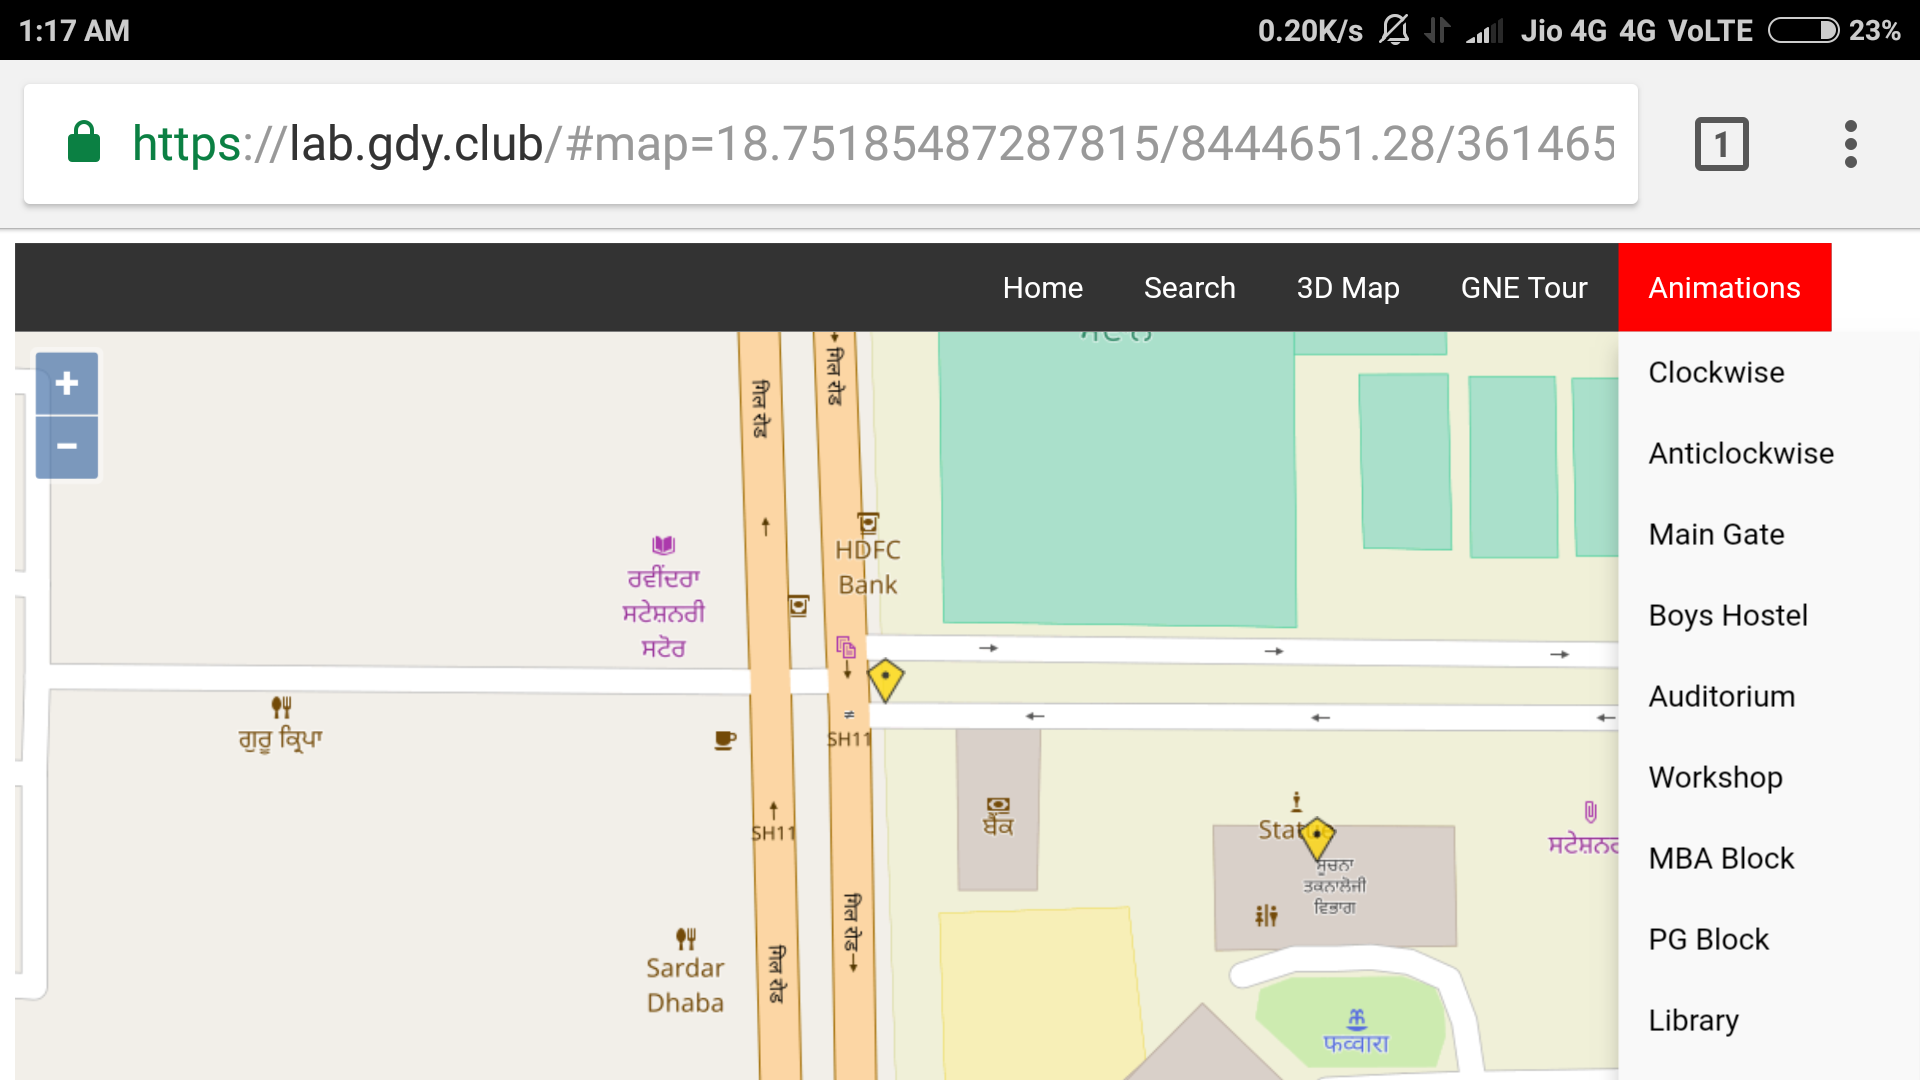
\includegraphics[width=0.7\textwidth]{input/images/animation.png}
\caption{Animation drop-down bar}
\end{figure}

\section{Testing}

